\chapter{Branched logic applied to reset}\label{chap:branched_logic}

In this section we look at applying branched logic to reset . By branched logic we mean the ability to take decisions in real time based on experimental outcomes such as measurements. By reset, we mean going into the ground state (0) of the superconducting qubit. In particular, we will be investigating how to optimize reset using branched logic. 

Results are an improvement of two orders of magnitude in the preparation fidelity in exchange of adding a second readout pulse. A Markov chain formalism is applied to reset. 

\section{The trivial way of performing reset} \label{sec:branched_logic}

Let's have a look at the most trivial way of performing a branched logic reset. One measures the state. If 1 is measured then a $\pi$-pulse is applied to get the qubit back into the 0 state. If 0 is measured, one does nothing. The state-diagram corresponding to this is shown on figure  \ref{fig:finite_branching}. Note that the algorithm will always stop and that both branches (left, right) have different run times. We define:
\begin{itemize}
    \item $p_{0|0}$ the probability to measure 0 while the qubit being in 0,
    \item $p_{1|1}$ the probability to measure 1 while the qubit being in 1,
    \item $p_{\pi|0}$ the probability to successfully performing a $\pi$-pulse while the qubit is in 0,  
    \item $p_{\pi|1}$ the probability to successfully performing a $\pi$-pulse while the qubit is in 1.
    \item $t_\mathrm{ro}$ ($t_\pi$) the time required to readout (apply a $\pi$-pulse to) the qubit

\end{itemize}

\begin{figure}[h]
    \centering
    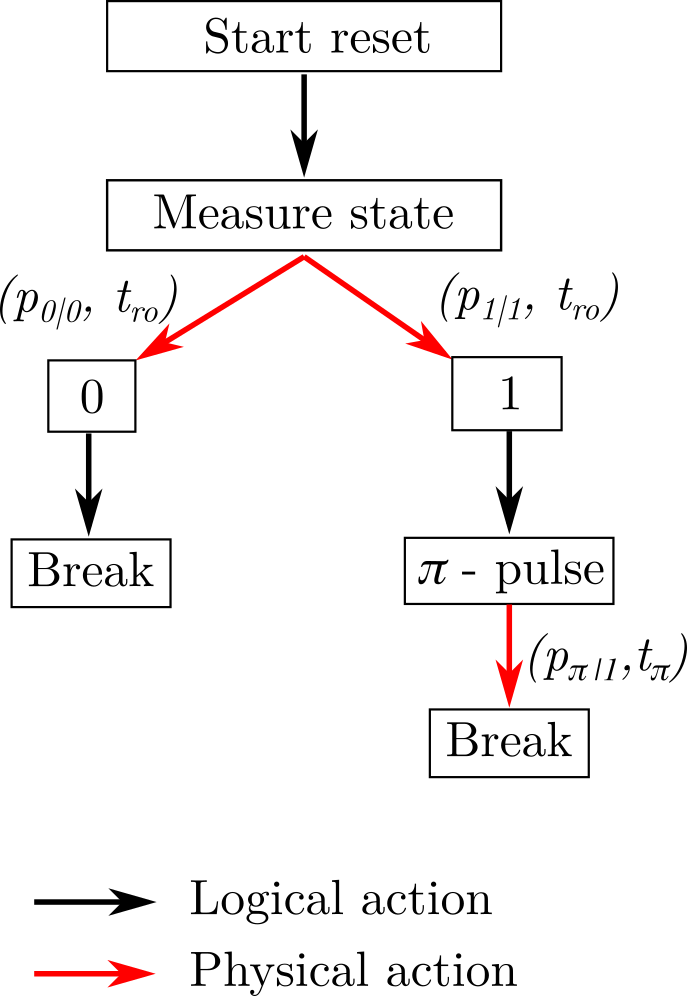
\includegraphics[width=0.5\textwidth]{pic/algorithmic_reset/finite_branching.png}
    \caption{Path-diagram for a simple reset}
    \label{fig:finite_branching}
\end{figure}

Now the question is how one can do better than the algorithm shown on figure \ref{fig:finite_branching}. For this, we want to add metrics characterizing our path-diagram. It becomes important to consider the initial state, which we assume to be $\ket{\Psi} \eqdef \alpha\ket{0} + \beta \ket{1}$.

A path is described by two properties:
\begin{itemize}
    \item \textbf{success probability}, capturing the probability $q_i$ that a path $i$ succeeds in ending in a 0 state. Note that $q_i$ is a function of initial conditions.
    \item \textbf{path time}, the time $t_i$ required to arrive at the end of the path.
\end{itemize}

A path diagram has again two properties we will be looking at: 
\begin{itemize}
    \item \textbf{total success probability}, capturing the probability $p_\textbf{success}$ the algorithm described by the diagram succeeds in resetting the qubit. 
    \item \textbf{expected termination time}, the expected time of termination $<t>$ of the algorithm.
\end{itemize}

For example, in our case one has two paths (left and right on figure \ref{fig:finite_branching}). The probabilities associated to success are given in table \ref{tab:path_finite_branching_table}.
 \begin{table}[h]
     \centering
     \begin{tabular}{c|c|c}
        Path & Success probability  & Time required \\ \hline
         Left & $q_\mathrm{left}= \abs{\alpha}^2p_{0|0}$ & $t_\mathrm{left} = t_{ro}$ \\
         Right & $q_\mathrm{right} = \abs{\beta}^2 p_{1|1}p_{\pi|1}$ & $t_\mathrm{right} = t_{ro} + t_\pi$
     \end{tabular}
     \caption{Table summarizing the success probabilities of paths shown on figure \ref{fig:finite_branching}. }
     \label{tab:path_finite_branching_table}
 \end{table}

Assuming for example $p_{0|0} = p_{1|1} = p_{\pi|} = p_{\pi|1} = 99\%, \abs{\alpha}^2  = 0.5$ one finds that $p_\text{success} = 98.505 \%$ and that $<t> =  t_{ro} + 0.495 t_\pi$.



\section{Branched logic approach to reset}
The algorithm presented in section \ref{sec:branched_logic} will always terminate after one run. However, in order to improve reset fidelity, one can decide to measure the qubit and applying a $\pi$-pulse \textit{while} seeing a 1 state. Once a ground state is measured, the algorithm stops. A path-diagram corresponding to this algorithm is given on figure \ref{fig:infinite_branching}.

\begin{figure}[h]
    \centering
    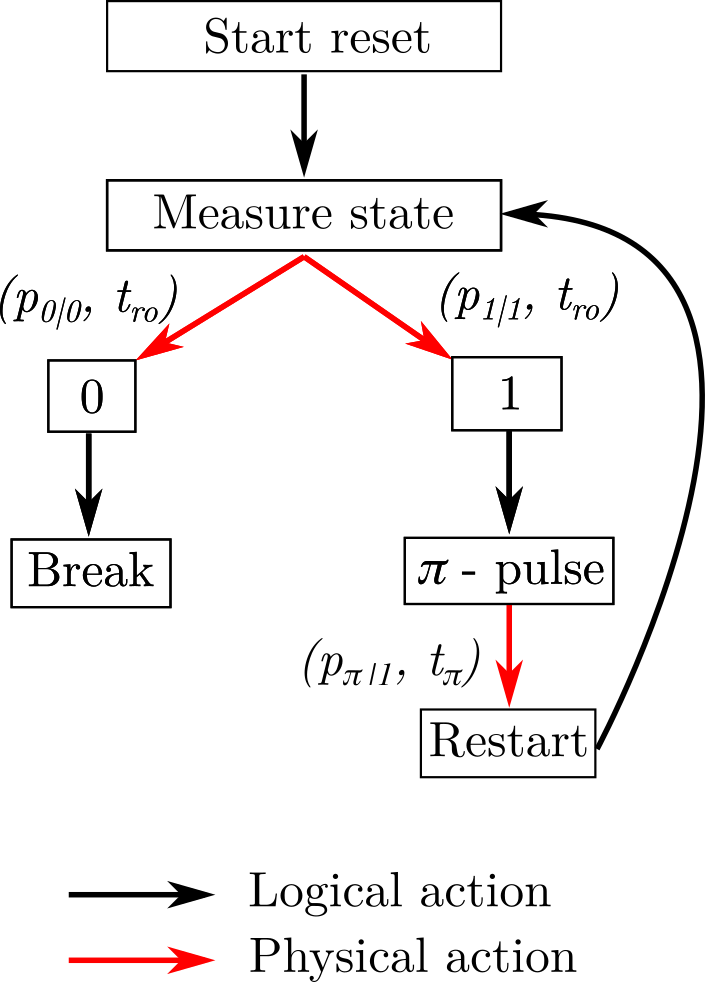
\includegraphics[width=0.5\textwidth]{pic/algorithmic_reset/infinite_branching.png}
    \caption{Ansatz on maximising state preparation fidelity}
    \label{fig:infinite_branching}
\end{figure}

Computing the probabilities and times associated to each path yields the results shown on table \ref{tab:path_infinite_branching_table}. It becomes obvious that manually computing paths and their probabilities is not possible anymore. In order to solve this, we introduce the Transition Matrix formalism.

 \begin{table}[H]
     \begin{tabular}{c|c|c|c}
       Path index $i$ & Path & Success probability $p_i$ & Time required \\ \hline
        0 & Left & $\abs{\alpha}^2 p_{0|0}$ & $t_{ro}$ \\
        1 &  Right, left & $\abs{\beta}^2p_{1|1}p_{\pi|1}p_{0|0}$ & $2t_{ro} + t_\pi$ \\
        2 &  Right, right, left & $\abs{\beta}^2 p_{1|1}^2 (1-p_{\pi|1}) p_{\pi|1} p_{0|0} + \abs{\alpha}^2 p_{1|0} p_{\pi|1} p_{1|1} p_{\pi|1} p_{0|0} $ & $3t_{ro} + 2t_\pi$ \\
         ... & ... & ... & ... \\
        n & (Right)$^n$, left & $p_{1|1}^np_{\pi|1}^np_{0|0} + \mathcal{O}(\epsilon)$ & $(n+1)t_{ro} + nt_\pi$ \\
        ... & ... & ... & ...
     \end{tabular}
     \caption{Table summarizing the success probabilities of paths shown on figure \ref{fig:infinite_branching}. $\epsilon$ is of the order of the probability that an operation goes wrong}
     \label{tab:path_infinite_branching_table}
 \end{table}
 
 \subsection{Transition matrix formalism}

% In fact what we are facing here is a decision problem.

We will introduce a formalism allowing us to compute success probabilities. 

%We have access to incomplete information about our system, and take actions accordingly. 
%% Insert picture knowledge => action => update knowledge. 

Our state diagram can be seen as a set of states. A state is defined by the knowledge of the qubit we have (ie. the measurement) and the actual state of the qubit. A list of states is given on table \ref{tab:states_branching1}.
 
 \begin{table}[h]
     \centering
     \begin{tabular}{c|c|c|c}
        State tag $s_i$ & State name & Description & Next action \\ \hline 
        $s_1$ & $0|0$  & 0 measured, qubit is in state 0 & \textbf{Break}\\ 
        $s_2$ & $0|1$  & 0 measured, qubit is in state 1 & \textbf{Break}\\ 
        $s_3$ & $1|0$  & 1 measured, qubit is in state 0 & Apply $\pi$-pulse, measure again\\ 
        $s_4$ & $1|1$  & 1 measured, qubit is in state 1 & Apply $\pi$-pulse, measure again
     \end{tabular}
     \caption{List of states of the path-diagram and of the actions taken.}
     \label{tab:states_branching1}
 \end{table}

After each round of algorithm one goes from one state to another with a certain probability. This is a Markov Chain setting. 

Note that the desired state is $s_1$. Once in $s_1$, we don't leave it anymore, it's an irreversible action. Similarly, reaching $s_2$ also is irreversible with the difference that being in $s_2$ means having failed the reset. To each path from $s_i$ to $s_j$ we can associate a transition probability $p_{j\leftarrow i} = (T)_{ji}$, giving us a Markov transition matrix $T$. In our case we have 
\begin{equation}
    T = \left(
\begin{array}{cccc}
 1 & 0 & {p_{0|0}} (1-{p_{\pi|0}}) & {p_{0|0}} {p_{\pi|1}} \\
 0 & 1 & (1-{p_{1|1}}) {p_{\pi|0}} & (1-{p_{1|1}}) (1-{p_{\pi|1}}) \\
 0 & 0 & (1-{p_{0|0}}) (1-{p_{\pi|0}}) & (1-{p_{0|0}}) {p_{\pi|1}} \\
 0 & 0 & {p_{1|1}} p_{\pi|0} & {p_{1|1}} (1-{p_{\pi|1}}) \\
\end{array}
\right)
\end{equation}

The matrix describes the evolution of the system. Defining a state vector $\Vec{P_k} = \bmat{P_{s_1}, P_{s_2}, P_{s_3}, P_{s_4}}^\top$ containing the probabilities $P_{s_i}$ of being in state $i$ after iteration $k$ we can investigate the time-evolution. Our initial state is given by 

\begin{equation}
    \Vec{P_0} = \bmat{\abs{\alpha}^2 p_{0|0}\\(\abs{\beta}^2) (1 - p_{1|1})\\\abs{\alpha}^2(1- p_{0|0})\\\abs{\beta}^2 p_{1|1}}. \label{eq:Pk}
\end{equation}

and the state after $k$ iterations is given by

\begin{equation}
   \Vec{P_k} = T^k \Vec{P_0}.
\end{equation}

\subsubsection{Computing the asymptotic evolution of the state-vector}

One can analytically compute the convergence of the scheme. Let $\left\{\vec e_i\right\}_{i\in \mathrm{states}}$ be the eigenvectors of $T$, and let $\left\{\lambda_i\right\}_{i\in \mathrm{states}}$ be the corresponding eigenvalues. Let $\left\{\gamma_i\right\}_{i\in \mathrm{states}}$ be such that 
\begin{equation}
    \vec P_0 = \sum_{i\in \mathrm{states}} \gamma_i \vec e_i.
\end{equation}

Then one has that 

\begin{equation}
    \vec P_k = T^k \vec P_0 =  \sum_{i\in \mathrm{states}} \gamma_i \lambda_i^k  \vec e_i.
\end{equation}

The eigenvalues of $T$ are (first analytically, then for $p_{0|0} = p_{1|1} = p_{\pi|} = p_{\pi|1} = 0.99$): 
\begin{eqnarray}
\lambda_1 = 1 \\
\lambda_2 = 1
\end{eqnarray}
\begin{equation}
\begin{split}
\lambda_3 = \frac{\sqrt{(p_{0|0} (-p_{\pi|0})+p_{0|0}+p_{1|1} (p_{\pi|1}-1)+p_{\pi|0}-1)^2-4 (p_{0|0}-1) p_{1|1} (p_{\pi|0}+p_{\pi|1}-1)}}{2} \\
+\frac{p_{0|0} (p_{\pi|0}-1)+p_{1|1} (-p_{\pi|1})+p_{1|1}-p_{\pi|0}+1}{2} \approx 0.1
\end{split}
\end{equation}

\begin{equation}
\begin{split}
\lambda_4 = \frac{-\sqrt{(p_{0|0} (-p_{\pi|0})+p_{0|0}+p_{1|1} (p_{\pi|1}-1)+p_{\pi|0}-1)^2-4 (p_{0|0}-1) p_{1|1} (p_{\pi|0}+p_{\pi|1}-1)}}{2} \\
+\frac{p_{0|0} (p_{\pi|0}-1)+p_{1|1} (-p_{\pi|1})+p_{1|1}-p_{\pi|0}+1}{2} \approx -0.09
\end{split}
\end{equation}

This shows that our scheme will exponentially converge into the $\mathrm{span}(\vec e_1, \vec e_2)$ subspace: repeatedly applying $T$ will exponentially suppress the components in $\mathrm{span}(\vec e_3, \vec e_4)$ as $\abs{\lambda_3}, \abs{\lambda_4} < 1$. We have that $\vec e_1 = \bmat{1, 0, 0, 0}^\top$ and $\vec e_2 = \bmat{0, 1, 0, 0}^\top$, corresponding to the state of the algorithm having terminated. This is reassuring as this means that our algorithm will terminate in a finite time with probability 1. 

The other eigenvectors can be found in the file \textit{path\_analysis.nb} (their analytical expression is - well - long). They are a linear combination of all components. %% add here exactly where to find it for future use

It is worth to note that the sum of components of $\vec e_1, \vec e_2$ equals 1, whereas for $\vec e_3, \vec e_4$ it equals 0. %% More discussion? 


We analytically find $\gamma_1, \gamma_2$ as they allow us to compute the asymptotic state. We find: 

\begin{equation}
    \lim_{k \to \infty}\Vec{P_k} = \lim_{k \to \infty} \sum_{i=1}^4 \gamma_i \vec e_i \lambda_i ^k = \bmat{\gamma_1 \\ \gamma_2\\0 \\ 0}.
\end{equation}

This not only gives us an asymptotic evolution but also a measure of how quickly we converge: the runtime of the algorithm is in $\mathcal{O} \left((\max_{i \in {3,4}}\abs{\lambda_i})^k\right)$. \textit{(not sure if one can say that this way - what I mean is that the probability of not having reset after k rounds decreases exponentially, the expected runtime can be easily computed as can be found below}

Furthermore, one can exactly compute probability of success and of failure: $\gamma_2$ is the probability that our scheme fails, $\gamma_1$ is the probability to succeed in the reset. Computing $\gamma_1$ and $\gamma_2$ for $\vec P_0$ as given in equation \ref{eq:Pk} one obtains: 

\begin{equation}
    \begin{split}
        \gamma_1 = \frac{p_{0|0} \left(\alpha ^2+p_{1|1} \left(p_{\pi|1}-\alpha ^2\right)\right)}{p_{0|0} (1-p_{1|1}) (1-p_{\pi|0})+p_{0|0} p_{1|1} p_{\pi|1}+ p_{\pi|0}(1-p_{1|1})},
    \end{split}
\end{equation}

\begin{equation}
    \begin{split}
       \gamma_2 = \frac{(1-p_{1|1}) \left(p_{0|0} \left(1-\alpha ^2-p_{\pi|0}\right)+p_{\pi|0}\right)}{p_{0|0} (1-p_{1|1}) (1-p_{\pi|0})+p_{0|0} p_{1|1} p_{\pi|1} + p_{\pi|0}(1-p_{1|1})}
    \end{split}
\end{equation}

with $\gamma_1 + \gamma_2 = 1$. This gives us an exact prediction of what the success probability of our reset scheme are, the probability of success being given by $\gamma_1$ and the probability of failure by $\gamma_2$.

Using the "toy values" $p_{0|0} = p_{1|1} = p_{\pi|} = p_{\pi|1} = 0.99$, one can compare success probabilities as a function of $\abs{\alpha}^2$. One finds:
\begin{equation}
    p_\text{success} = 98.99 \% + 0.010099 \cdot \abs{\alpha}^2 \overset{\abs{\alpha}^2 = \frac{1}{2}}{=} 99.48 \%
\end{equation}



Note that there is a 1\% increase compared to the previous scheme. 

The main error source could to be investigated thoroughly, but intuitively one can see that the main error contribution happens at the first step when wrongfully measuring a 0 state. The success probability can be further enhanced as will be discussed in section \ref{sec:double_readout}.  

\subsubsection{Computing termination time}

Using Mathematica, it is straightforward to compute $\Vec{P_k}$ for a set of starting values. An example of an evolution is given on figure \ref{fig:p_k}.

\begin{figure}[h]
    \centering
    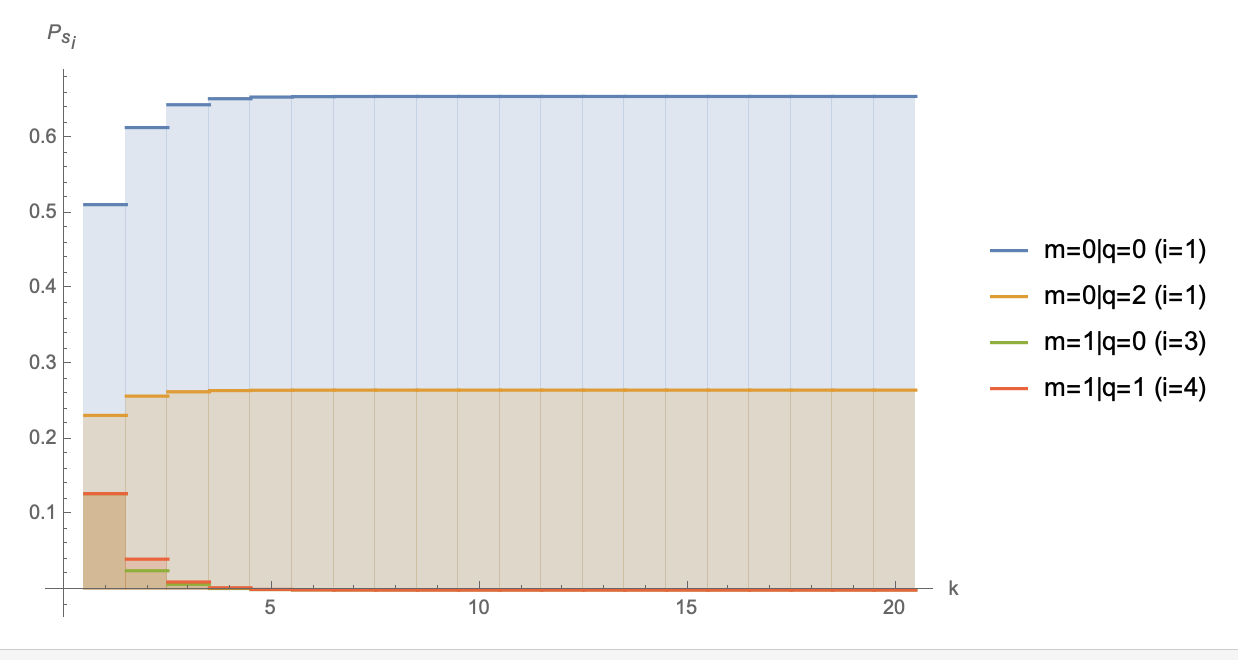
\includegraphics[width=0.6\textwidth]{state_prop_evol_i=4.png}
    \caption{\textbf{(to be
    changed: this figure was generated with a small bug in the code. Starting values should be adjusted for a nicer picture)}. Note that there is a residual population in the $s_2$ state, which means our reset is not working perfectly. }
    \label{fig:p_k}
\end{figure}

This allows computing the expected time of reset $<t>$: 

\begin{equation}
\begin{split}
    < t > = \sum_{k = 0 }^\infty \underbrace{\left[P_{s_1,k+1} + P_{s_2,k+1} - (P_{s_1,k} + P_{s_2,k})\right]}_{\text{Probability of terminating after } k+1 \text{ steps}}\underbrace{(t_{ro} + t_\pi)(k+1)}_{\text{time process took}} - \underbrace{t_{\pi}}_{\text{no pulse once 0 measured}}\\ 
\end{split}
\end{equation}

This can be further simplified to 

\begin{equation}
\begin{split}
    < t > = \sum_{k = 0 }^\infty \underbrace{\left[\gamma_1 + \gamma_2 - \gamma_3\lambda_3^k((\vec{e_3})_1 + (\vec{e_3})_2) - \gamma_4\lambda_4^k((\vec{e_4})_1 + (\vec{e_4})_2) \right]}_{\text{Probability of terminating after } k+1 \text{ steps}}\underbrace{(t_{ro} + t_\pi)(k+1)}_{\text{time process took}} \\
    - \underbrace{t_{\pi}}_{\text{no pulse once 0 measured}}\\ 
\end{split}
\end{equation}

Which are all values we have computed previously. Unfortunately, getting the analytical solution is not very instructive, so plugging some numbers into the equations helps us seeing clearer. Assuming again $p_{0|0} = p_{1|1} = p_{\pi|} = p_{\pi|1} = 0.99, \abs{\alpha}^2  = 0.5$, we have that: 

\begin{equation}
    <t> = t_{ro} + (0.9947 - \abs{\alpha}^2 0.9548) (t_{ro} + t_\pi) \overset{\abs{\alpha}^2 = \frac{1}{2}}{=} t_{ro} + 0.5173(t_{ro} + t_\pi)
\end{equation}

where one sees that on average the time difference between this and the previous scheme is approximately $t_{ro}$. So for the price of one more readout one gets around 1\% improvement for our "toy" values.  





\section{Improving the reset probability} \label{sec:double_readout}

The main source of error in the previously proposed scheme is when wrongly measuring a 0. To avoid this happening one can decide reading out a second time to ensure that we start with a correct state.

A state diagram is shown on figure \ref{fig:double_infinite_branching}. 

\begin{figure}[h]
    \centering
    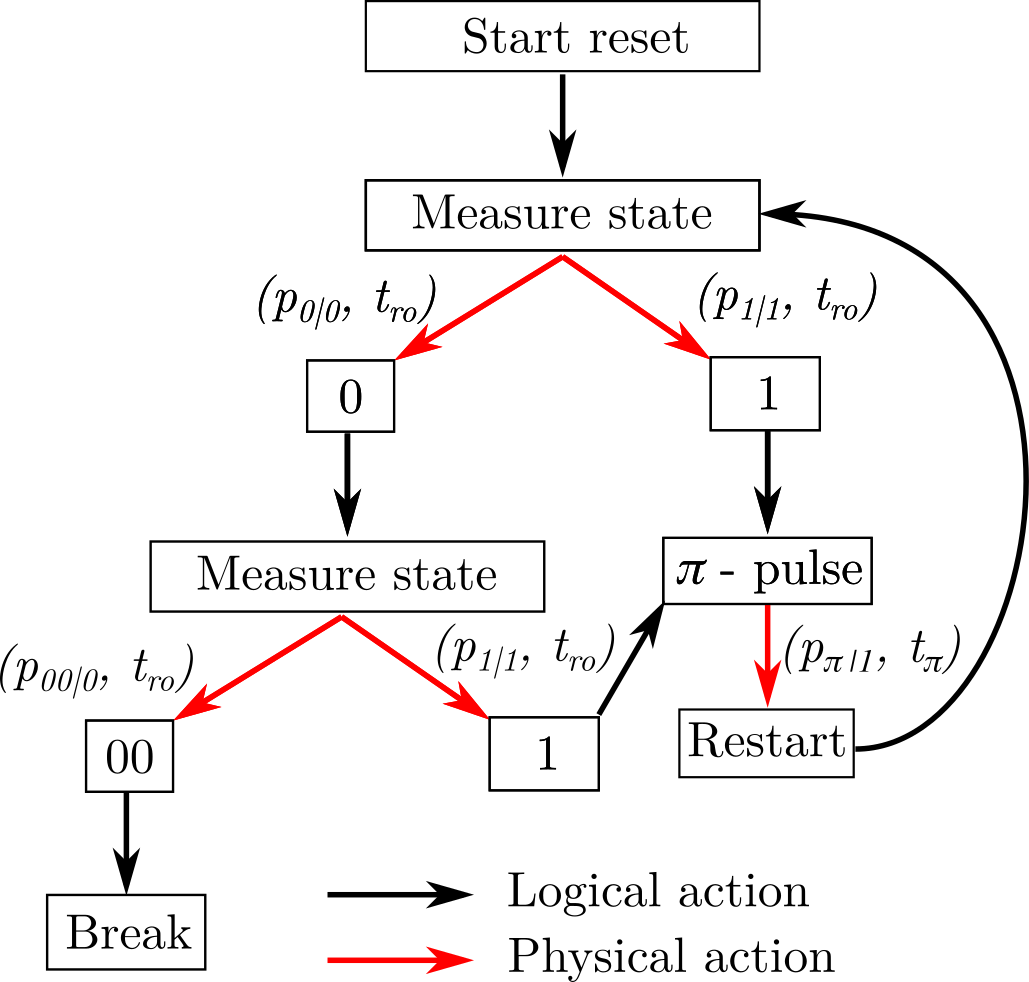
\includegraphics[width=0.5\textwidth]{pic/algorithmic_reset/double_infinite_branching.png}
    \caption{Caption}
    \label{fig:double_infinite_branching}
\end{figure}

A list of states is given on table \ref{tab:states_branching2}

 
 \begin{table}[h]
     \centering
     \begin{tabular}{c|c|c|c}
        State tag $s_i$ & State name & Description & Next action \\ \hline 
        $s_1$ & $0|0$  & 0 measured, qubit is in state 0 & Measure again \\ 
        $s_2$ & $0|1$  & 0 measured, qubit is in state 1 & Measure again \\ 
        $s_3$ & $1|0$  & 1 measured, qubit is in state 0 & Apply $\pi$-pulse, measure again \\ 
        $s_4$ & $1|1$  & 1 measured, qubit is in state 1 & Apply $\pi$-pulse, measure again \\
        $s_5$ & $00|0$  & 0 measured twice, qubit is in state 0 & \textbf{Break} (successful) \\
        $s_6$ & $00|1$  & 0 measured twice, qubit is in state 1 & \textbf{Break} (unsuccessful) \\
        
     \end{tabular}
     \caption{List of states of the path-diagram for improved reset fidelty}
     \label{tab:states_branching2}
 \end{table}


Applying the same treatment as before, but now in a 6-dimensional state-space one has: 

\begin{equation}
    \Vec{P_0} = \bmat{\abs{\alpha}^2 p_{0|0}\\(\abs{\beta}^2) (1 - p_{1|1})\\\abs{\alpha}^2(1- p_{0|0})\\\abs{\beta}^2 p_{1|1} \\ 0 \\ 0}. \label{eq:Pk6}
\end{equation}
%% Markov transition Matrix

\begin{equation}
    T = \bmat{0 & 0 & p_{0|0}(1-p_{\pi|0}) & p_{0|0} p_{\pi|1} & 0 & 0 \\ 
    0 & 0 & (1-p_{1|1})p_{\pi|0} & (1-p_{1|1})(1-p_{\pi|1}) & 0 & 0 \\ 
    (1-p_{0|0}) & 0 & (1-p_{0|0})(1-p_{\pi|0}) & (1-p_{0|0})p_{\pi|1} & 0 & 0 \\
    0 & p_{1|1} & p_{1|1}p_{\pi|0} & p_{1|1}(1-p_{\pi|1}) & 0 & 0\\ 
    p_{0|0} & 0 & 0 & 0 & 1 & 0 \\
    0 & (1-p_{1|1}) & 0 & 0 & 0 & 1}
\end{equation}

$T$ again has the same properties as before, namely that we have two unity eigenvalues corresponding to the final states $s_5$ and $s_6$. The eigenvalues corresponding to the other eigenstates are $|\cdot| < 1$. One can, using the same method as previously, compute the probabilities of success. All files describing the calculations can be found in the files \textit{path\_analysis.nb} and \textit{path\_analysis.m}. Note that computing eigenvalues and eigenvectors analytically for the $6\times6$ matrix $T$ is not realistic anymore, therefore it was chosen to simply leave $t_{ro}$ and $t_{\pi}$ as symbolic variables when computing $<t>$. Note also that the formula for $<t>$ slightly changes: 

\begin{equation}
\begin{split}
    < t > = \sum_{k = 0 }^\infty \underbrace{\left[P_{s_5,k+1} + P_{s_6,k+1} - (P_{s_5,k} + P_{s_6,k})\right]}_{\text{Probability of terminating after } k+1 \text{ steps}}\underbrace{(t_{ro} + t_\pi)(k+1)}_{\text{time process took}} \\ + \underbrace{t_{ro}}_{\text{initialization time}} - \underbrace{t_{\pi}}_{\text{no pulse once 0 measured}}\\ 
\end{split}
\end{equation}

Results are the following, again for our toy model with probabilities $p_{0|0} = p_{1|1} = p_{\pi|} = p_{\pi|1} = 0.99$. 

\begin{eqnarray}
p_\text{success} = 99.99\% + 1.01\e{-4} \abs{\alpha}^2  \overset{\abs{\alpha}^2 = \frac{1}{2}}{=} 99.995 \% \\
<t> = (2.0709 - 1.02 \abs{\alpha}^2)(t_\pi + t_{ro}) + t_{ro} \overset{\abs{\alpha}^2 = \frac{1}{2}}{=} 1.5609(t_\pi + t_{ro}) + t_{ro}
\end{eqnarray}

Here it becomes clear that by paying a small time tribute one can significantly improve the reset success probability.

\section{Optimization choices}

A reset protocol is usually followed by an experiment, which will last a certain amount of time $t_\mathrm{exp}$.
Two optimisation routes can be taken:
\begin{enumerate}
    \item maximize the number of experiments starting with a successful reset, which means taking the state-diagram maximizing
    \begin{equation}
        \sum_{i \in \mathrm{paths}} q_i(t_i + t_\mathrm{exp}), \label{eq:pathtime-optimizer}
    \end{equation}
    \item minimize the number of experiments starting with a wrongly reset state, which means taking the diagram maximizing
    \begin{equation}
        \sum_{i \in \mathrm{paths}}  q_i,
    \end{equation}
\end{enumerate} 

where $q_i$ is the probability to take path $i$ successfully (ie. that one takes path $i$ and that you end up in the ground state) and $t_i$ the length of the path. 

Option 1 means maximizing the number of successful experiments while paying the price of starting sometimes with a wrong state. This option could be interesting if one can post-select on wrongly prepared states or if one can live with errors. If one decides to run an algorithm where the correctness of the answer is easily checked (e.g. factorisation of prime numbers) this option should be favoured.

Option 2 means trying everything you can do to be absolutely sure to start in the right state. This is the option maximizing experiment fidelity, to be chosen whenever one cannot post-select on the outcome of an experiment. 

Note that in the limit of $t_i \ll t_\mathrm{exp} \forall i \in \mathrm{paths}$, option 1 becomes equivalent to option 2. Also, this reasoning generalizes to any case where one has a trade-off between speed and accuracy. 

Finally, it would be interesting to compute numbers for equation \ref{eq:pathtime-optimizer}. One could for example numerically compute: 

\begin{equation}
\begin{split}
    < t > = \sum_{k = 0 }^\infty \underbrace{\left[P_{s_5,k+1} - P_{s_5,k})\right]}_{\text{Probability of success after } k+1 \text{ steps}}\cdot \underbrace{(t_{ro} + t_\pi)(k+1)}_{\text{time process took}} \\ + \underbrace{t_{ro}}_{\text{initialization time}} - \underbrace{t_{\pi}}_{\text{no pulse once 0 measured}}\\ 
\end{split}
\end{equation}

this has not been further investigated but could provide useful for short experiments where the correctness of the outcome can be assessed. 